% ==========================================================================
\chapter{Jin--Xin 松弛系统的源项分裂}
% ==========================================================================

前两章的分析建立在“对流显式、扩散隐式”的分裂之上。本章把同一套语言推广到另一类刚性系统——Jin--Xin 松弛系统。这里的刚性不再来自空间导数，而来自源项中的 $1/\varepsilon$；分裂的对象也从扩散算子变成了源项。第 \ref{sec:jinxin-model} 节介绍模型与平衡极限；第 \ref{sec:jinxin-splitting} 节给出两种源项分裂；第 \ref{sec:jinxin-stability} 节推导 $2\times2$ 放大矩阵并作谱分析；第 \ref{sec:jinxin-numerics} 节给出数值对比；第 \ref{sec:jinxin-discussion} 节讨论结果的含义。

\section{Jin--Xin 松弛系统}
\label{sec:jinxin-model}

对无粘 Burgers 方程 $u_t+f(u)_x=0$，$f(u)=u^2/2$，Jin 与 Xin 引入松弛系统\cite{jinxin1995}
\begin{equation}
  \begin{cases}
    u_t+v_x=0,\\[4pt]
    v_t+a^2u_x=-\dfrac{1}{\varepsilon}\bigl(v-f(u)\bigr),
  \end{cases}
  \label{eq:jinxin}
\end{equation}
其中 $v$ 为松弛变量，$a>0$ 为常数，$\varepsilon>0$ 为松弛参数。当 $\varepsilon\to0$ 时，源项强迫 $v\to f(u)$，第二个方程退化为 $v=f(u)$，第一个方程变为
\begin{equation}
  u_t+f(u)_x=0.
  \label{eq:equilibrium}
\end{equation}
因此，松弛系统是对原守恒律的一种逼近：它把非线性通量 $f(u)$ 替换为一个线性双曲系统加一个刚性源项。

\subsection{平衡极限与次特征条件}

对 \eqref{eq:jinxin} 作 Chapman--Enskog 展开。设 $v=f(u)+\varepsilon v_1+O(\varepsilon^2)$，代入第二个方程并保留首阶项，得
\begin{equation}
  v_1=-\bigl(f'(u)u_t+a^2u_x\bigr).
  \label{eq:chapman-enskog}
\end{equation}
再利用 $u_t=-v_x=-f(u)_x+O(\varepsilon)$，可得一阶修正。要使松弛系统在 $\varepsilon\to0$ 时稳定地收敛到 \eqref{eq:equilibrium}，特征速度 $a$ 必须不小于平衡通量的特征速度：
\begin{equation}
  a\ge\max_u|f'(u)|=\max_u|u|.
  \label{eq:subcharacteristic}
\end{equation}
这就是次特征条件。本文取 $a=1$，初始数据 $u_L=1$、$u_R=0$，因此条件恰好取等号。

松弛系统的优点是通量线性：$u$ 的通量为 $v$，$v$ 的通量为 $a^2u$。这使得我们可以直接套用有限体积的 Rusanov 通量，而不必处理非线性 Riemann 问题。代价是源项具有 $1/\varepsilon$ 的刚性，必须用隐式或渐近保持方法处理。

\subsection{线性化}

设 $\bar u$ 为常数状态，$b=f'(\bar u)=\bar u$。在 $(\bar u,f(\bar u))$ 附近线性化 \eqref{eq:jinxin}：
\begin{equation}
  \begin{pmatrix}\delta u\\ \delta v\end{pmatrix}_t
  +\begin{pmatrix}0&1\\ a^2&0\end{pmatrix}
  \begin{pmatrix}\delta u\\ \delta v\end{pmatrix}_x
  =\frac{1}{\varepsilon}
  \begin{pmatrix}0&0\\ b&-1\end{pmatrix}
  \begin{pmatrix}\delta u\\ \delta v\end{pmatrix}.
  \label{eq:jinxin-linear}
\end{equation}
源项的 Jacobian 为
\begin{equation}
  \bJ=\frac{1}{\varepsilon}
  \begin{pmatrix}0&0\\ b&-1\end{pmatrix}.
  \label{eq:source-jacobian}
\end{equation}
它有一个零特征值（对应 $u$ 的守恒模态）和一个 $-1/\varepsilon$ 的特征值（对应 $v$ 的快速松弛模态）。刚性正来自后者的模 $1/\varepsilon$。

\section{两种源项分裂}
\label{sec:jinxin-splitting}

对 \eqref{eq:jinxin} 采用 IMEX-Euler：输运项显式，源项按不同方式分裂。设 $\mu=\Delta t/\varepsilon$，并记 $\bL$ 为 Rusanov 离散后的输运算子。

\subsection{策略 A：源项全隐式}

策略 A 把整个源项放在新时刻：
\begin{equation}
  \begin{cases}
    u^{n+1}=u^n+\Delta t\,\bL_u(u^n,v^n),\\[4pt]
    v^{n+1}=v^n+\Delta t\,\bL_v(u^n,v^n)
    -\mu\left(v^{n+1}-f(u^{n+1})\right).
  \end{cases}
  \label{eq:strategy-A}
\end{equation}
整理得
\begin{equation}
  v^{n+1}=\frac{v^n+\Delta t\,\bL_v(u^n,v^n)+\mu f(u^{n+1})}{1+\mu}.
  \label{eq:strategy-A-v}
\end{equation}
由于 $u^{n+1}$ 已由第一个方程显式算出，第二个方程不需要非线性迭代；所谓“全隐式”，是指 $v^{n+1}$ 与 $f(u^{n+1})$ 都在新时刻取值。

\subsection{策略 B：仅隐式化线性刚性部分}

策略 B 把源项写成“线性刚性部分 $-$ 非线性部分”：
\begin{equation}
  -\frac{1}{\varepsilon}\bigl(v-f(u)\bigr)
  =-\frac{1}{\varepsilon}v+\frac{1}{\varepsilon}f(u).
  \label{eq:source-split}
\end{equation}
只对 $-v/\varepsilon$ 作隐式处理，$f(u)/\varepsilon$ 在旧时刻取值：
\begin{equation}
  \begin{cases}
    u^{n+1}=u^n+\Delta t\,\bL_u(u^n,v^n),\\[4pt]
    v^{n+1}=v^n+\Delta t\,\bL_v(u^n,v^n)
    -\mu v^{n+1}+\mu f(u^n).
  \end{cases}
  \label{eq:strategy-B}
\end{equation}
整理得
\begin{equation}
  v^{n+1}=\frac{v^n+\Delta t\,\bL_v(u^n,v^n)+\mu f(u^n)}{1+\mu}.
  \label{eq:strategy-B-v}
\end{equation}
与策略 A 相比，式 \eqref{eq:strategy-B-v} 只是把 $f(u^{n+1})$ 换成了 $f(u^n)$。在实现上，这一差别很小；但在稳定性上，它却是本质的。

\subsection{一个看似无害的差别}

如果不看输运项，只分析源项本身，策略 A 与 B 的放大矩阵都是
\begin{equation}
  \begin{pmatrix}1&0\\ \dfrac{\mu b}{1+\mu}&\dfrac{1}{1+\mu}\end{pmatrix},
  \label{eq:source-only}
\end{equation}
特征值为 $1$ 与 $1/(1+\mu)$。两者都稳定，且快速模态都被 $1/(1+\mu)$ 压掉。因此，\textbf{仅看源项}无法区分 A 与 B；必须把输运项与源项耦合起来，使用完整的 $2\times2$ 放大矩阵。这正是双变量稳定性函数思想在松弛系统中的体现。

\section{线性稳定性分析}
\label{sec:jinxin-stability}

\subsection{输运算子的符号}

对 \eqref{eq:jinxin} 的线性输运算符
\begin{equation}
  \bA=\begin{pmatrix}0&1\\ a^2&0\end{pmatrix},
  \label{eq:transport-matrix}
\end{equation}
采用 Rusanov 通量，其 Fourier 符号为
\begin{equation}
  \bL(\xi)=-\frac{\ii\sin\xi}{\Delta x}\bA
  -\frac{a(1-\cos\xi)}{\Delta x}\bI.
  \label{eq:transport-symbol}
\end{equation}
令
\begin{equation}
  g=c(1-\cos\xi),\qquad h=\frac{c}{a}\sin\xi,\qquad c=\frac{a\Delta t}{\Delta x},
  \label{eq:g-h}
\end{equation}
则 $\Delta t\bL(\xi)=-\bI g-\ii h\bA$。于是
\begin{equation}
  \bI+\Delta t\bL(\xi)=
  \begin{pmatrix}1-g&-\ii h\\ -\ii a^2h&1-g\end{pmatrix}.
  \label{eq:I-plus-L}
\end{equation}

\subsection{策略 A 的放大矩阵}

由 \eqref{eq:strategy-A}，先算 $u^{n+1}=u^n+\Delta t\bL_u$，再算
\begin{equation}
  (1+\mu)v^{n+1}=v^n+\Delta t\bL_v+\mu b\,u^{n+1}.
\end{equation}
写成矩阵形式：
\begin{equation}
  \bM_A=
  \begin{pmatrix}
    1-g & -\ii h\\[4pt]
    \dfrac{\mu b(1-g)-\ii a^2h}{1+\mu}
    & \dfrac{(1-g)-\ii\mu b h}{1+\mu}
  \end{pmatrix}.
  \label{eq:M-A}
\end{equation}

\subsection{策略 B 的放大矩阵}

同理，
\begin{equation}
  \bM_B=
  \begin{pmatrix}
    1-g & -\ii h\\[4pt]
    \dfrac{-\ii a^2h+\mu b}{1+\mu}
    & \dfrac{1-g}{1+\mu}
  \end{pmatrix}.
  \label{eq:M-B}
\end{equation}
两者的差别只在第二行：A 的 $(2,1)$ 元含 $\mu b(1-g)$，$(2,2)$ 元含 $-\ii\mu b h$；B 的 $(2,1)$ 元含 $\mu b$，$(2,2)$ 元没有 $\mu b h$ 项。正是这些 $O(\mu)$ 的项，在刚性极限下决定了稳定性。

\subsection{刚性极限}

令 $\mu\to\infty$，得
\begin{align}
  \bM_A^\infty&=
  \begin{pmatrix}
    1-g&-\ii h\\ b(1-g)&-\ii b h
  \end{pmatrix},
  \label{eq:M-A-inf}\\
  \bM_B^\infty&=
  \begin{pmatrix}
    1-g&-\ii h\\ b&0
  \end{pmatrix}.
  \label{eq:M-B-inf}
\end{align}
$\bM_A^\infty$ 的两行成比例，特征值为 $0$ 与 $1-g-\ii bh$。因此
\begin{equation}
  \rho(\bM_A^\infty)=|1-g-\ii bh|.
  \label{eq:rho-A}
\end{equation}
取 $b=a$，有
\begin{equation}
  |1-g-\ii ah|^2=(1-g)^2+a^2h^2
  =1-2c(1-c)(1-\cos\xi)\le1,\qquad 0\le c\le1.
  \label{eq:rho-A-bound}
\end{equation}
所以策略 A 在 $\CFL\le1$ 时稳定，且当 $c<1$ 时除 $\xi=0$ 外都有严格小于 $1$ 的衰减。这一结论与 $\mu$ 无关，说明 A 是渐近保持的：无论 $\varepsilon$ 多小，稳定性都不退化。

$\bM_B^\infty$ 的特征值满足
\begin{equation}
  \lambda^2-(1-g)\lambda+\ii bh=0.
  \label{eq:char-B}
\end{equation}
其谱半径不能写成简单的闭式。取 $b=a$，对 $\xi$ 作数值扫描，可以得到如下结果。

\begin{itemize}[leftmargin=2.2em]
  \item 当 $c\le1/3$ 时，$\rho(\bM_B^\infty)\le1$；
  \item 当 $c>1/3$ 时，$\rho(\bM_B^\infty)>1$，且超出量随 $c$ 增大而增大；
  \item 临界值 $1/3$ 与 $\mu$ 无关：在 $\mu=0.1$ 到 $10^{4}$ 的范围内，临界 CFL 稳定在 $0.33334$ 至 $0.33344$。
\end{itemize}

表 \ref{tab:jinxin-critical} 给出了不同 $\mu$ 下的临界 CFL。可以看到，即使 $\mu$ 只有 $0.1$（源项并不算“刚性”），临界值也已经降到 $1/3$。这说明策略 B 的缺陷不是“刚性太强”造成的，而是分裂结构本身造成的：把 $f(u)$ 滞后一个时刻，破坏了输运模态与源模态之间的精确平衡，产生了一个伪增长模。

\begin{table}[htbp]
  \centering
  \caption{策略 B 的临界 CFL 随 $\mu$ 的变化（谱半径扫描）}
  \label{tab:jinxin-critical}
  \begin{tabular}{lcccccc}
    \toprule
    $\mu$ & $0.1$ & $1$ & $10$ & $10^2$ & $10^3$ & $10^4$ \\
    \midrule
    $\CFL_{\rm crit}$ & $0.33344$ & $0.33335$ & $0.33334$ & $0.33334$ & $0.33334$ & $0.33334$ \\
    \bottomrule
  \end{tabular}
\end{table}

图 \ref{fig:jinxin-stability} 给出了两种策略的谱半径随 CFL 的变化。左图中，策略 A 的曲线在 $\CFL\le1$ 时都不超过 $1$，说明它稳定；右图中，策略 B 的曲线在 $\CFL>1/3$ 后迅速上升，且 $\mu$ 越大上升越快。当 $\mu\to\infty$ 时，曲线趋近于一条与 $\mu$ 无关的极限曲线，其起点正是 $1/3$。

\begin{figure}[htbp]
  \centering
  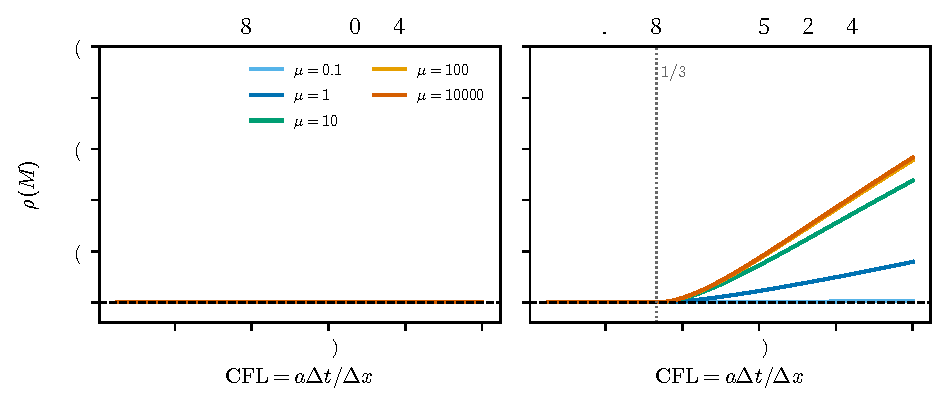
\includegraphics[width=0.96\textwidth]{jinxin_stability.pdf}
  \caption{Jin--Xin 系统两种源项分裂的谱半径。(a) 策略 A；(b) 策略 B。两图颜色对应相同的 $\mu$；虚线为 $\rho=1$，点线为 $\CFL=1/3$。}
  \label{fig:jinxin-stability}
\end{figure}

\subsection{为什么是 \texorpdfstring{$1/3$}{1/3}}

$1/3$ 的出现可以从低频展开理解。取 $b=a$，则 $bh=ah=c\sin\xi$，慢特征值近似为
\begin{equation}
  \lambda_{\rm slow}\approx\frac{\ii bh}{1-g}
  =\frac{\ii c\sin\xi}{1-c(1-\cos\xi)}.
\end{equation}
在 $\xi\to0$ 时展开：
\begin{equation}
  \lambda_{\rm slow}
  =\ii c\xi\left[1+\left(\frac{c}{2}-\frac{1}{6}\right)\xi^2+O(\xi^4)\right].
\end{equation}
方括号中的修正项在 $c=1/3$ 处变号：当 $c>1/3$ 时，低频端的模长开始超过 $1$，数值扫描显示最不稳定模态位于 $\xi/\pi\approx0.02$ 至 $0.2$，并随 $c$ 增大向高波数移动；当 $c<1/3$ 时，整个低频带的模长不超过 $1$。$c=1/3$ 正是这一低频不稳定带的起点。严格的全局证明需要对 $|\lambda|$ 作更细致的估计，本文不展开；数值扫描在 $10^{-10}$ 的精度内把临界值定在 $1/3$，足以支持后续讨论。

\section{数值实验}
\label{sec:jinxin-numerics}

在 $[-1,1]$ 上求解 \eqref{eq:jinxin}，取 $N=400$、$a=1$、$\varepsilon=10^{-4}$、$t=1$，初始数据为 Riemann 问题
\begin{equation}
  u_0(x)=\begin{cases}1,&x<0,\\0,&x>0,\end{cases}
  \qquad v_0(x)=f(u_0(x)).
  \label{eq:jinxin-riemann}
\end{equation}
精确解为以速度 $1/2$ 向右传播的激波。分别用策略 A 与 B 在 $\CFL=0.3,0.5,0.7$ 下计算，结果列于表 \ref{tab:jinxin-numerics}。

\begin{table}[htbp]
  \centering
  \caption{Jin--Xin 松弛系统的数值结果（$N=400$，$\varepsilon=10^{-4}$，$t=1$）}
  \label{tab:jinxin-numerics}
  \begin{tabular}{cccccc}
    \toprule
    策略 & $\CFL$ & 状态 & $L^1$ 误差 & $\max|u|$ & 平衡残差 \\
    \midrule
    A & $0.3$ & 稳定 & $3.292\times10^{-3}$ & $1.000$ & $3.97\times10^{-3}$ \\
    A & $0.5$ & 稳定 & $3.122\times10^{-3}$ & $1.000$ & $3.98\times10^{-3}$ \\
    A & $0.7$ & 稳定 & $2.938\times10^{-3}$ & $1.000$ & $4.12\times10^{-3}$ \\
    \midrule
    B & $0.3$ & 稳定 & $2.886\times10^{-3}$ & $1.013$ & $2.56\times10^{-2}$ \\
    B & $0.5$ & 振荡 & $2.791\times10^{-3}$ & $1.043$ & $5.67\times10^{-2}$ \\
    B & $0.7$ & 失稳 & --- & $4.45\times10^{1}$ & $7.60\times10^{2}$ \\
    \bottomrule
  \end{tabular}
\end{table}

\begin{figure}[htbp]
  \centering
  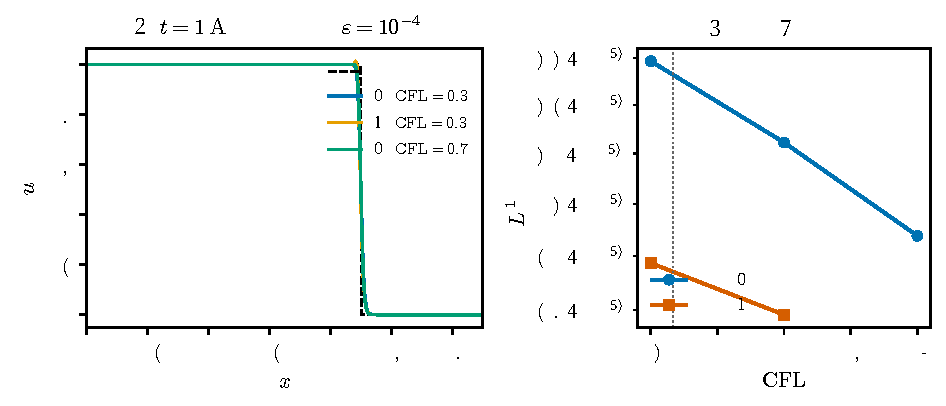
\includegraphics[width=0.94\textwidth]{jinxin_numerics.pdf}
  \caption{Jin--Xin 系统的数值对比（$\varepsilon=10^{-4}$，$t=1$）。(a) 两种策略在 $\CFL=0.3$ 的解，以及策略 A 在 $\CFL=0.7$ 的解；(b) $L^1$ 误差随 CFL 的变化。策略 B 在 $\CFL=0.7$ 时失稳，误差无定义，故其曲线止于 $\CFL=0.5$。}
  \label{fig:jinxin-numerics}
\end{figure}

表 \ref{tab:jinxin-numerics} 与图 \ref{fig:jinxin-numerics} 显示了清晰的对比：

第一，策略 A 在三个 CFL 下都稳定，$L^1$ 误差在 $2.9\times10^{-3}$ 至 $3.3\times10^{-3}$ 之间，且随 CFL 增大略有下降。这与第四章的“数值扩散随 CFL 增大而减小”的现象一致。平衡残差 $\max|v-f(u)|$ 约为 $4\times10^{-3}$，与 $L^1$ 误差同量级，说明 A 在每个时间步结束时基本把解拉回平衡流形。

第二，策略 B 在 $\CFL=0.3$ 时稳定，$L^1$ 误差甚至略小于 A（$2.886\times10^{-3}$ 对 $3.292\times10^{-3}$）；但它的平衡残差为 $2.56\times10^{-2}$，是 A 的 $6.5$ 倍。到 $\CFL=0.5$，B 的 $L^1$ 误差仍略小，但 $\max|u|$ 已增至 $1.043$，平衡残差增至 $5.67\times10^{-2}$，出现了明显的振荡；此时谱半径已略大于 $1$，只是增长较慢，尚未在 $t=1$ 内发散。到 $\CFL=0.7$，B 完全失稳，$\max|v|$ 达到 $2.3\times10^{2}$，计算中止。

第三，B 的“低 CFL 下略准”并不矛盾。B 的源项滞后一个时刻，相当于对 $f(u)$ 作了一次显式外推，这在低 CFL 下可能偶然抵消一部分数值耗散；但它破坏了平衡流形的约束，随着 CFL 增大，误差迅速积累并最终失稳。A 的平衡残差始终保持在 $4\times10^{-3}$，说明它的稳定性是有物理基础的，而不是误差抵消的结果。

\section{讨论}
\label{sec:jinxin-discussion}

\subsection{容许性与 L-稳定}

用第四章的语言，策略 A 是容许的：它在 $\CFL\le1$ 时沿刚性射线稳定，且快速模态的放大因子为 $1/(1+\mu)\to0$，因此是 L-稳定的。策略 B 不是容许的：虽然它的快速模态也被 $1/(1+\mu)$ 压掉，但慢模态的放大矩阵 $\bM_B^\infty$ 在 $\CFL>1/3$ 时谱半径大于 $1$，且这一限制不随 $\mu\to\infty$ 消失。因此，B 的失稳不是“快速模态没压住”，而是“慢模态被源项的滞后项污染了”。

\subsection{与渐近保持性质的关系}

渐近保持（AP）要求格式在 $\varepsilon\to0$ 时稳定地收敛到平衡系统的格式。策略 A 在 $\varepsilon\to0$ 时给出 $v^{n+1}\to f(u^{n+1})$，下一步的 $u$ 更新使用 $f(u^{n+1})$，因此极限格式是平衡系统的一阶显式格式。策略 B 给出 $v^{n+1}\to f(u^n)$，极限格式用的是上一步的 $f$，相当于多了一个时间步的滞后。两者都是一阶 AP，但 B 的滞后破坏了输运模态与源模态之间的平衡结构，导致 CFL 限制从 $1$ 降到 $1/3$。这说明：AP 性质本身不足以保证稳定性；分裂的结构同样重要。

\subsection{计算代价}

在本文的顺序分裂中，$u^{n+1}$ 先由显式输运算出，因此策略 A 计算 $f(u^{n+1})$ 并不比 B 计算 $f(u^n)$ 贵。两者的每步计算量几乎相同。若把源项与输运完全耦合求解，A 需要解一个非线性方程组，代价会更高；此时可以采用线性化的全隐式（Newton 一步）或 IMEX Runge--Kutta 方法。无论哪种实现，本文关于“滞后 $f(u)$ 会破坏容许性”的结论都适用。

\subsection{向粘性情形的推广}

若在 $u$ 方程中加入 $\nu u_{xx}$，则松弛系统变为
\begin{equation}
  \begin{cases}
    u_t+v_x=\nu u_{xx},\\[4pt]
    v_t+a^2u_x=-\dfrac{1}{\varepsilon}\bigl(v-f(u)\bigr).
  \end{cases}
  \label{eq:jinxin-viscous}
\end{equation}
对扩散项可以采用第三章的 $\theta$ 分裂，对源项可以采用本章的 A/B 分裂。两类刚性——扩散刚性 $1/\Delta x^2$ 与源项刚性 $1/\varepsilon$——可以分别处理，稳定性分析仍然是“双变量”的，只是变量从二维增加到三维（$z_E,z_I,\mu$）。本文不展开这一推广，但它说明了本文框架的可迁移性。

\section{本章小结}

本章把双变量稳定性函数的语言推广到 Jin--Xin 松弛系统，比较了两种源项分裂。主要结论如下：
\begin{enumerate}[label=(\arabic*),leftmargin=2.4em]
  \item 仅分析源项无法区分策略 A 与 B；必须使用包含输运耦合的 $2\times2$ 放大矩阵。
  \item 策略 A 在 $\CFL\le1$ 时稳定，且与 $\mu$ 无关；其刚性极限的特征值为 $0$ 与 $1-g-\ii bh$，模不超过 $1$。
  \item 策略 B 的临界 CFL 为 $1/3$，且该值在 $\mu=0.1$ 到 $10^{4}$ 的范围内几乎不变。B 的失稳源于 $f(u)$ 的滞后破坏了慢模态的结构。
  \item 数值实验验证了上述结论：A 在 $\CFL=0.7$ 时仍稳定，B 在 $\CFL=0.7$ 时失稳；B 在低 CFL 下虽然略准，但平衡残差随 CFL 迅速增大。
\end{enumerate}
这些结果说明，“容许分裂”不仅是扩散分裂的设计准则，也是松弛系统源项分裂的设计准则。
